\documentclass{article}

% if you need to pass options to natbib, use, e.g.:
%     \PassOptionsToPackage{numbers, compress}{natbib}
% before loading neurips_2024


% ready for submission
\usepackage[final]{neurips_2024}


% to compile a preprint version, e.g., for submission to arXiv, add add the
% [preprint] option:
%     \usepackage[preprint]{neurips_2024}


% to compile a camera-ready version, add the [final] option, e.g.:
%     \usepackage[final]{neurips_2024}


% to avoid loading the natbib package, add option nonatbib:
%    \usepackage[nonatbib]{neurips_2024}


\usepackage[utf8]{inputenc} % allow utf-8 input
\usepackage[T1]{fontenc}    % use 8-bit T1 fonts
\usepackage{hyperref}       % hyperlinks
\usepackage{url}            % simple URL typesetting
\usepackage{booktabs}       % professional-quality tables
\usepackage{amsfonts}       % blackboard math symbols
\usepackage{nicefrac}       % compact symbols for 1/2, etc.
\usepackage{microtype}      % microtypography
\usepackage{xcolor}         % colors
\usepackage{graphicx}
\usepackage{amsmath}

\title{Improving Human Pose Estimation: A Comparative Analysis of SimpleBaseline and Stacked Hourglass Networks Using the MPII Dataset and PCKh-0.5 Metric}


% The \author macro works with any number of authors. There are two commands
% used to separate the names and addresses of multiple authors: \And and \AND.
%
% Using \And between authors leaves it to LaTeX to determine where to break the
% lines. Using \AND forces a line break at that point. So, if LaTeX puts 3 of 4
% authors names on the first line, and the last on the second line, try using
% \AND instead of \And before the third author name.


\author{%
  DongJoo Hwang \\
  AI Researcher \\
  Aiffel Research 10th \\
  \texttt{hdjcool@gmail.com} \\
}

\begin{document}


\maketitle


\begin{abstract}
Human pose estimation is a critical technology designed to predict human posture by detecting keypoints, such as joints and essential body parts. This study evaluates and compares the performance of two prominent models: the Stacked Hourglass Network and the SimpleBaseline model, using the MPII Human Pose Dataset. The evaluation utilizes the PCKh@0.5 metric (Percentage of Correct Keypoints with head-normalized threshold) to measure prediction accuracy.

Our findings demonstrate that the SimpleBaseline model consistently outperforms the Stacked Hourglass Network in both quantitative and qualitative evaluations. The SimpleBaseline model demonstrates lower training and validation loss and improves accuracy across all keypoints.

These results highlight SimpleBaseline’s efficiency and accuracy, establishing it as an ideal choice for real-world human pose estimation tasks. Future work will explore optimization strategies and additional architectural enhancements to further improve performance.

\textbf{Keywords}: Human Pose Estimation, SimpleBaseline, Stacked Hourglass Network, MPII Dataset, PCKh@0.5, Keypoint Detection
\end{abstract}


\section{Introduction}


Detecting human posture through keypoint-based human pose estimation has become a fundamental task in computer vision due to its relevance in applications like healthcare and human-computer interaction. It serves as a critical technology in various applications, including healthcare monitoring, sports performance analysis, and human-computer interaction (HCI). Despite significant advancements, pose estimation continues to face challenges such as occlusions, complex poses, and variations in image conditions.
This study compares two widely-used models for human pose estimation: Stacked Hourglass Network and SimpleBaseline. By leveraging the MPII Human Pose Dataset and evaluating with the PCKh@0.5 metric, we aim to identify the strengths and weaknesses of each approach and demonstrate the practical advantages of SimpleBaseline over Stacked Hourglass Network.

\section{Background}
\label{gen_inst}

Human pose estimation involves detecting keypoints such as shoulders, elbows, and knees from images to estimate the human body’s structure. Keypoint detection accuracy directly influences downstream tasks, including activity recognition, motion tracking, and augmented reality.
Challenges in Pose Estimation:

\begin{itemize}
\item Occlusions: Keypoints hidden by objects or other body parts.
\item Complex Poses: Unusual body positions causing ambiguity.
\item Scale Variations: Differences in person size due to camera distance.


\end{itemize}

To address these challenges, deep learning models such as Stacked Hourglass Network and SimpleBaseline have been introduced.

\section{Related Works}
\label{headings}

\subsection{Stacked Hourglass Network:}
The Stacked Hourglass Network, operating as a multi-scale feature extraction model, utilizes stacked hourglass modules to capture fine-grained details across various resolutions. While effective, it faces challenges of high computational costs and training instability.

\subsection{SimpleBaseline Model:}
The SimpleBaseline model simplifies the architecture by employing a ResNet backbone for feature extraction and a deconvolutional decoder to predict keypoint heatmaps. This design enhances computational efficiency and prediction accuracy.

This study compares these two models on the MPII Human Pose Dataset using the PCKh@0.5 metric to provide clarity on their respective strengths and weaknesses.

\section{Method}
\label{others}

\subsection{Dataset: MPII Human Pose Dataset}

In this study, we use the MPII Human Pose Dataset to train and evaluate our human pose estimation models. The dataset comprises over 25,000 images and more than 40,000 human instances, with each human body represented by 16 keypoints, including the head, shoulders, elbows, wrists, hips, knees, and ankles. Additionally, the dataset captures a variety of poses, angles, background complexities, and occlusions, making it suitable for real-world evaluation.

\subsection{Baseline Model: Stacked Hourglass Network}

The Stacked Hourglass Network is designed to predict human poses through multi-resolution feature extraction and a symmetrical structure. This network stacks multiple Hourglass modules to capture multi-scale features, enabling the prediction of complex poses and fine details. However, the network suffers from high computational costs and training difficulties due to its deep architecture. To address these limitations, we propose the SimpleBaseline model.

\subsection{Proposed Model: SimpleBaseline}

SimpleBaseline adopts an encoder-decoder architecture to provide an efficient and intuitive approach to pose estimation. The model employs ResNet as the backbone to effectively extract image features and then predicts keypoint heatmaps using a decoder network. 
The key improvements of SimpleBaseline include:

\begin{itemize}
\item Simplified Architecture: Removing unnecessary complexity to improve computational efficiency.
\item Accurate Feature Extraction: Leveraging ResNet’s strong representational power for precise feature extraction.
\end{itemize}

These improvements contribute to faster training speed and higher accuracy in pose prediction.

\subsection{Training Details}

The training process utilizes a customized Mean Squared Error (MSE) loss function to minimize pixel-wise errors between the ground truth heatmaps and the predicted heatmaps. Notably, a weight of 81 is assigned to keypoint regions in the ground truth to emphasize their importance during training. The loss function is defined as:

\[
\text{Loss} = \frac{1}{\text{global\_batch\_size}} \sum (\text{labels} - \text{outputs})^2 \cdot \text{weights}
\]

This weighting mechanism ensures the prioritization of keypoints during the training process, maintaining a balanced emphasis across the heatmap.

Data augmentation techniques such as random rotation, horizontal flipping, and scaling adjustments were applied to enhance the model’s generalization performance.

\subsection{Evaluation Metric: PCKh@0.5}

The PCKh@0.5 (Percentage of Correct Keypoints with head-normalized threshold) metric is used to evaluate the model’s performance. This metric determines whether a predicted keypoint is correct by measuring the Euclidean distance between the predicted and ground truth keypoints. A prediction is considered correct if the distance is within 50\% of the head length.

Keypoint-specific PCKh@0.5 scores are calculated to provide a detailed performance assessment, ensuring robustness against variations in human poses and scaling factors.

\subsection{Preprocessing Pipeline}

To efficiently preprocess input images and keypoint data, we designed a Preprocessor class. The pipeline consists of the following steps:

\begin{enumerate}
    \item Image Resizing and Normalization:
    \begin{enumerate}
        \item Original images are resized to (256, 256, 3).
        \item Pixel values are normalized to the range [-1, 1].
    \end{enumerate}
    \item Region of Interest (ROI) Cropping:
    \begin{enumerate}
        \item The ROI is determined based on the minimum/maximum keypoint coordinates and body height.
        \item A random margin is added during training to enable data augmentation.
    \end{enumerate}
    \item Keypoint Normalization:
    \begin{enumerate}
        \item After ROI cropping, keypoint coordinates are normalized to a range of (0, 1).
    \end{enumerate}
    \item Gaussian Heatmap Generation:
    \begin{enumerate}
        \item Each keypoint is converted into a 64x64 Gaussian Heatmap.
        \item Invisible keypoints (visibility == 0) are excluded from the heatmap.
        \item The heatmap consists of 16 channels, one for each keypoint.
    \end{enumerate}
    \item Dataset Parsing
    \end{enumerate}

This preprocessing pipeline ensures that the data is clean, normalized, and properly formatted for effective model training and evaluation.

\section{Results – Model Comparison (Stacked Hourglass Network vs. SimpleBaseline)}

\subsection{Experimental Setup}
In this study, we compared the Stacked Hourglass Network and SimpleBaseline models to evaluate their performance on the MPII Human Pose Dataset. Both models were evaluated using the PCKh@0.5 metric, and training loss, validation loss, and keypoint-specific PCKh values were analyzed.
Here are the main settings for the experiment:

\begin{itemize}
\item \textbf{Number of Epochs:} 20
\item  \textbf{Optimizer:} Adam Optimizer
\item  \textbf{Learning Rate:} 0.0007
\item  \textbf{Evaluation Metric:} PCKh-0.5
\end{itemize}

\subsection{Quantitative Comparison}

\begin{table}[htpb]
    \centering
    \caption{Comparison of Training and Validation Performance Between Stacked Hourglass and SimpleBaseline Models}
    \label{tab:model_comparison}
    \begin{tabular}{|l|c|c|c|c|}
        \hline
        \textbf{Model} & \textbf{Train Loss} & \textbf{Val Loss} & \textbf{Average PCKh (Train)} & \textbf{Average PCKh (Val)} \\ \hline
        Stacked Hourglass & 0.9959 & 1.1075 & 0.0002457 & 0.0002457 \\ \hline
        SimpleBaseline    & 0.2172 & 0.2917 & 0.12825   & 0.12825   \\ \hline
    \end{tabular}
\end{table}
Table 1 provides a comparative analysis of training loss, validation loss, and average PCKh scores for the Stacked Hourglass Network and SimpleBaseline models, evaluated on the MPII Human Pose Dataset.
\begin{figure}[htbp]
  \centering
  \begin{minipage}{0.48\textwidth}
    \centering
    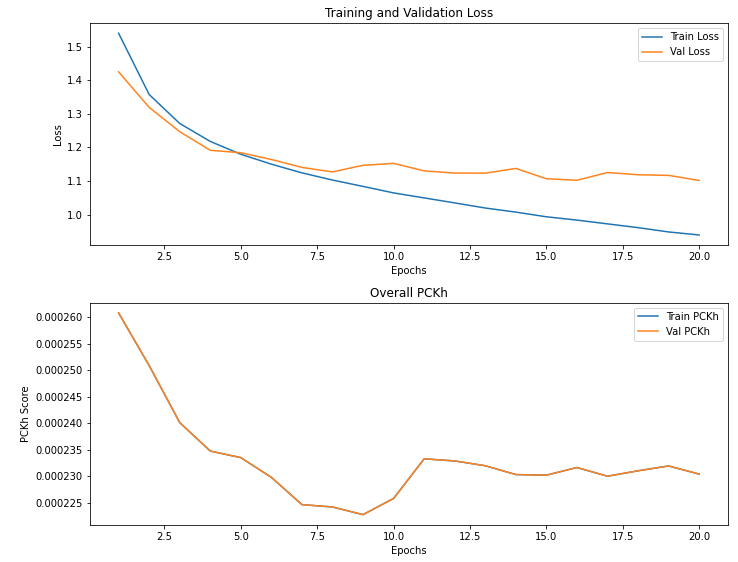
\includegraphics[width=0.9\textwidth]{figure1.png}
        \caption{Training and Validation Loss and Overall PCKh for Stacked Hourglass Network}
        \label{fig:stacked_hourglass_loss}
  \end{minipage}
  \hfill
  \begin{minipage}{0.48\textwidth}
    \centering
    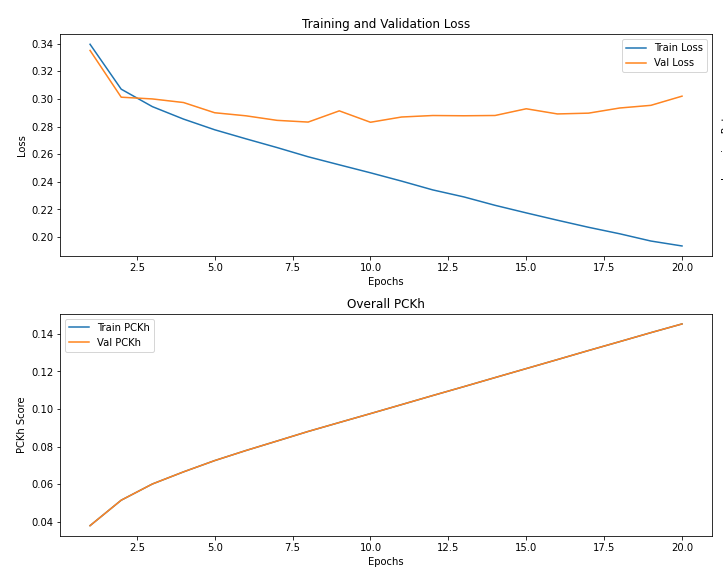
\includegraphics[width=0.9\textwidth]{figure2.png}
    \caption{Training and Validation Loss and Overall PCKh for SimpleBaseline}
    \label{fig:simplebaseline_loss}
  \end{minipage}
\end{figure}

Figure 1 illustrates the training and validation loss curves (top) along with the overall PCKh scores (bottom) over 20 epochs for the Stacked Hourglass Network model.

Figure 2 illustrates the training and validation loss curves (top) along with the overall PCKh scores (bottom) over 20 epochs for the SimpleBaseline model.

\begin{table}[htpb]
    \centering
    \caption{Model Training Time per Epoch and Loss}
    \label{tab:model_training_time}
    \begin{tabular}{|l|c|c|c|}
        \hline
        \textbf{Model} & \textbf{Epoch} & \textbf{Training Time (seconds)} & \textbf{Training Loss} \\ \hline
        \textbf{Stacked Hourglass} & 1 & 1783.27 & 1.5394 \\ \cline{2-4}
                                 & 2 & 1659.95 & 1.3574 \\ \cline{2-4}
                                 & 3 & 1648.77 & 1.2713 \\ \cline{2-4}
                                 & 4 & 1641.31 & 1.2179 \\ \cline{2-4}
                                 & 5 & 1703.94 & 1.1797 \\ \cline{2-4}
        \textbf{Average}         &   & \textbf{1687.45} & \textbf{1.3131} \\ \hline
        \textbf{SimpleBaseline}  & 1 & 828.63 & 0.3396 \\ \cline{2-4}
                                 & 2 & 816.67 & 0.3071 \\ \cline{2-4}
                                 & 3 & 816.83 & 0.2944 \\ \cline{2-4}
                                 & 4 & 839.62 & 0.2854 \\ \cline{2-4}
                                 & 5 & 823.38 & 0.2777 \\ \cline{2-4}
        \textbf{Average}         &   & \textbf{825.03} & \textbf{0.3008} \\ \hline
    \end{tabular}
\end{table}
Table 2 demonstrates the superiority of SimpleBaseline in terms of both training efficiency and loss minimization. With 49\% less training time per epoch and significantly lower training loss, SimpleBaseline outperforms the Stacked Hourglass Network in practical scenarios requiring both efficiency and accuracy.

Analysis:
\begin{itemize}
\item  Average PCKh: SimpleBaseline demonstrated a significant improvement in the average PCKh score across both training and validation phases.
\item Loss: The SimpleBaseline model achieved lower training and validation losses compared to the Stacked Hourglass Network, indicating better convergence.
\end{itemize}

The training times and performance of the Stacked Hourglass Network and SimpleBaseline model were compared over 5 epochs on the same dataset. The results, summarized in Table 2, indicate that SimpleBaseline requires 825.03 seconds per epoch on average, compared to 1687.45 seconds for the Stacked Hourglass Network. This 49\% reduction in training time highlights SimpleBaseline’s computational efficiency, which is attributed to its simpler architecture leveraging a ResNet backbone and deconvolution-based decoder.
In addition to faster training, SimpleBaseline achieves a consistently lower training loss, averaging 0.3008, compared to 1.3131 for the Stacked Hourglass Network. This suggests that SimpleBaseline not only trains faster but also optimizes better, making it a preferable choice for scenarios requiring efficient and accurate human pose estimation.

\subsection{Keypoint-wise PCKh Comparison}

\begin{table}[htpb]
    \centering
    \caption{Keypoint-wise PCKh-0.5 Performance Comparison Between Stacked Hourglass Network and SimpleBaseline}
    \label{tab:keypoint_comparison}
    \begin{tabular}{|c|c|c|l|}
        \hline
        \textbf{Keypoint} & \textbf{Stacked Hourglass (Val)} & \textbf{SimpleBaseline (Val)} & \textbf{Description} \\ \hline
        Keypoint 1  & 0.00017223 & 0.06383678 & Top of the head     \\ \hline
        Keypoint 2  & 0.00018018 & 0.07470323 & Neck                \\ \hline
        Keypoint 3  & 0.00029677 & 0.0686248  & Right shoulder      \\ \hline
        Keypoint 4  & 0.00022258 & 0.0677345  & Left shoulder       \\ \hline
        Keypoint 5  & 0.00018283 & 0.07642024 & Right elbow         \\ \hline
        Keypoint 6  & 0.00013249 & 0.0663752  & Left elbow          \\ \hline
        Keypoint 7  & 0.00025172 & 0.11232644 & Right wrist         \\ \hline
        Keypoint 8  & 0.00024907 & 0.21215156 & Left wrist          \\ \hline
        Keypoint 9  & 0.00024377 & 0.2322761  & Right hip           \\ \hline
        Keypoint 10 & 0.00025702 & 0.18190514 & Left hip            \\ \hline
        Keypoint 11 & 0.00025172 & 0.1150106  & Right knee          \\ \hline
        Keypoint 12 & 0.00026232 & 0.13591945 & Left knee           \\ \hline
        Keypoint 13 & 0.00021993 & 0.13631955 & Right ankle         \\ \hline
        Keypoint 14 & 0.00028352 & 0.1368283  & Left ankle          \\ \hline
        Keypoint 15 & 0.00031532 & 0.13261527 & Right eye           \\ \hline
        Keypoint 16 & 0.00023317 & 0.11382618 & Left eye            \\ \hline
    \end{tabular}
\end{table}

Table 3 presents a detailed comparison of PCKh-0.5 scores for each keypoint between the Stacked Hourglass Network and the SimpleBaseline model. The PCKh-0.5 metric measures the accuracy of each keypoint prediction, normalized by head length. Higher values indicate better prediction accuracy.

Analysis:
\begin{itemize}
\item The SimpleBaseline model outperformed the Stacked Hourglass Network across all keypoints.
\item   Significant improvements were observed in keypoints like left wrist (Keypoint 8), right hip (Keypoint 9), and left hip (Keypoint 10).
\end{itemize}

\section{Discussion}
\begin{figure}[htbp]
    \centering
    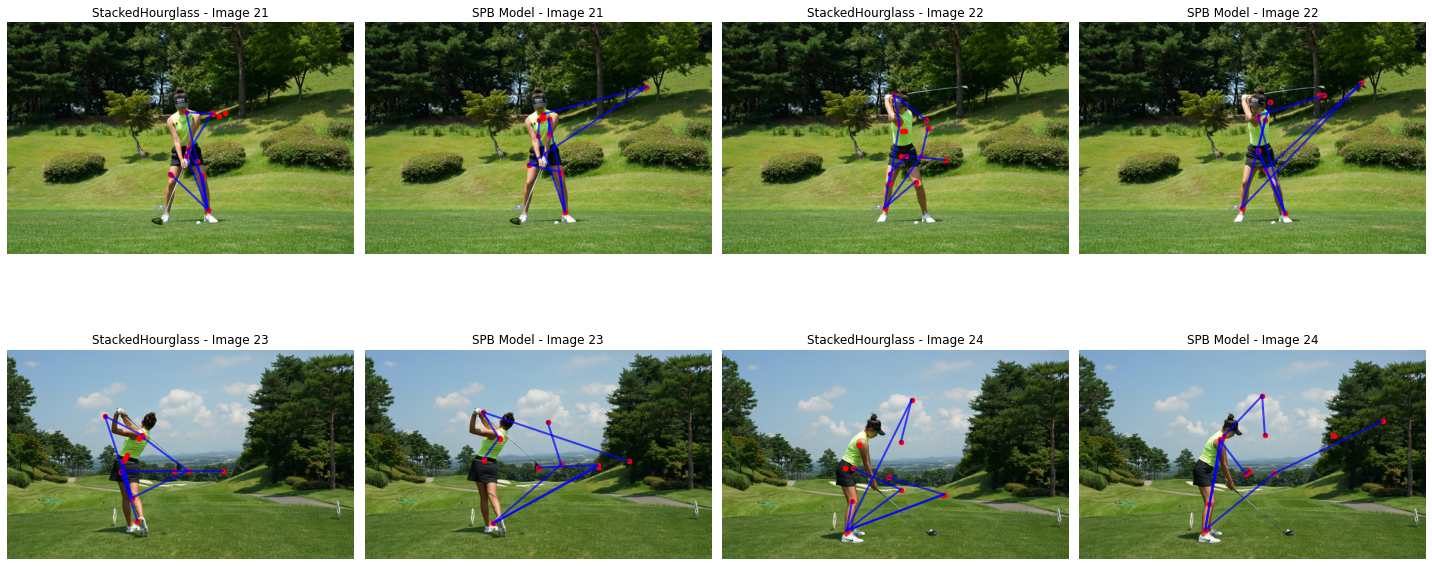
\includegraphics[width=0.8\textwidth]{figure3.png}
    \caption{Qualitative Comparison of Keypoint Predictions Between Stacked Hourglass Network and SimpleBaseline}
    \label{fig:keypoint_presictions}
\end{figure}

The qualitative evaluation (as shown in Figure 3) illustrates the challenges of both the Stacked Hourglass Network and the SimpleBaseline model in accurately predicting human pose keypoints during complex and dynamic scenarios. Despite achieving reasonable results for certain keypoints, significant issues persist: 
\begin{enumerate}
    \item \textbf{Prediction Errors}: Both models show significant inaccuracies, especially in complex poses or scenarios involving occlusion, which are critical for practical applications like sports analysis. 
    \item \textbf{Incomplete Skeleton Structures}: The connections between keypoints tend to be incomplete or misaligned, leading to unnatural skeletal representations. These errors limit the applicability of these models in real-world scenarios where reliability is crucial. 
    \end{enumerate}

\section{Conclusion and Future Work}

The SimpleBaseline model showed higher accuracy and robustness compared to the Stacked Hourglass Network and also proved to be more efficient. However, the above results suggest that further advances in human pose estimation models are needed to meet the requirements of real-world applications. Future research should focus on bridging the gap between research performance and practical utility. By simultaneously achieving accurate predictions and real-time performance, models should be deployable in a variety of practical applications, such as sports analytics.

\section*{References}
[1] Tompson, J., Goroshin, R., Jain, A., LeCun, Y., \& Bregler, C.\ (2015). Efficient Object Localization Using Convolutional Networks. In {\it Proceedings of the IEEE Conference on Computer Vision and Pattern Recognition (CVPR)}, pp.\ 648–656. New York University. Retrieved from \url{https://arxiv.org/abs/1411.4280}.

[2] Newell, A., Yang, K., \& Deng, J.\ (2016). Stacked Hourglass Networks for Human Pose Estimation. In {\it Proceedings of the European Conference on Computer Vision (ECCV)}, pp.\ 483–499. University of Michigan, Ann Arbor. Retrieved from \url{https://arxiv.org/abs/1603.06937}.

[3] Xiao, B., Wu, H., \& Wei, Y.\ (2018). Simple Baselines for Human Pose Estimation and Tracking. In {\it Proceedings of the European Conference on Computer Vision (ECCV)}, pp.\ 466–481. Microsoft Research Asia and University of Electronic Science and Technology of China. Retrieved from \url{https://arxiv.org/abs/1804.06208}.

\end{document}